\section{Experiment Design}

In this section, we present how to effectively find possible global optimal programs in our experiment. 

\subsection{High-level Workflow}
Figure~\ref{fig:workflow} depicts the high-level workflow of our experimental design. Given a program \po{}, we first design universal transformations (\ie, $\mathcal{D}$ in Definition~\ref{def:prob}) and use them to transform \po{} into new programs \pd{}. Then, we apply existing phase ordering methods to \pd{}. In the performance estimation phase, we estimate the performance of \pd{}. When $t(\pd) \geq T$ ($T$ is an anticaped execution time defined in Definition~\ref{def:prob}), we go back to \pd{} and do the phase ordering again. This procedure will continue until the performance is better than the original program or it reaches a threshold.
Finally, we compile the program and produce the optimal code. 
It is worth noting that the backward step relies on the phase ordering method we choose. An exhaustive search solution for phase ordering will guarantee the production of optimal programs with sufficient performance gain, so the backward step is unnecessary. However, machine learning-based methods~\cite{ashouri2017micomp} require the step because they cannot guarantee this property.

We discuss the major components below:
\begin{itemize}[leftmargin=*]
	% \item \textbf{\textit{Original Programs.}}\, Existing studies often opt for programs generated by random code generators (\eg, CSmith~\cite{yang2011finding}) to identify optimization bugs in compilers. However, in this work, we focus on real-world programs, which helps translate our findings to practice more seamlessly. 
	\item \textbf{\textit{Universal Transformation.}}\, The universal transformation transforms an original program \po{} to transformed programs \pd{} by the transformation set $\mathcal{D}$ (Definition~\ref{def:prob}). The transformation set consists of a sequence of transformations, including deoptimizations and performance-irrelevant transformations. Deoptimizations are constructed by inverting existing compiler optimizations. In order to apply transformation in $\mathcal{D}$, we design several strategies: \wyc{todo}, all of which are discussed in the next section.
	\item \textbf{\textit{Phase Ordering.}}\, We use the existing phase ordering tool \gfjc{TODO} to generate the best-optimized program for each transformed program. 
	% \item \textbf{\textit{Performance Checking.}}\, \wyc{maybe use runtime profilers?} Our performance checking encompasses two aspects: code size and expected runtime. We employ static performance checkers to evaluate whether the performance of the optimized program \pdc is less than $T$. If such a situation is observed, we conclude that an optimal program has been found.
\end{itemize}



\begin{figure}[t]
	\centering
	\Description{The experimental workflow, illustrating the process of benchmark selection, solver integration, and the evaluation pipeline for COMPASS.}
	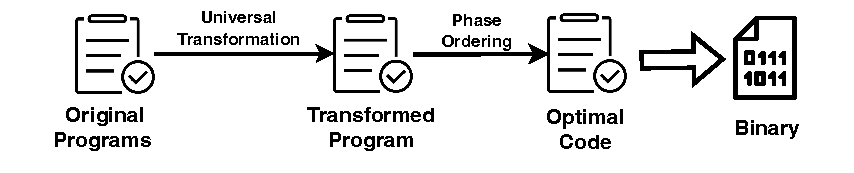
\includegraphics[width=0.7\linewidth]{pics/workflow.pdf}
	\caption{Overview of our approach.}
	\label{fig:workflow}
\end{figure}

\subsection{Universal Transformation}
% As explained in Section~\ref{sec:form}, there are potentially two approaches to generating programs with varying levels of efficiency. Considering our research is centered on real-world programs and compilers, which typically offer limited scope for optimization, we choose to perform universal transformations on an original program to produce more variants. 

Universal transformations consist of deoptimizations and optimization-irrelevant transformations.
We first discuss how to design deoptimizations and optimization-irrelevant transformations, and then illustrate how we apply universal transformations.
% We first introduce basic definitions for deoptimization, then discuss how to design deoptimizations, and finally, we give an algorithm for illustrating how to apply deoptimizations.




% To mutate a given seed program $P$ to $P'$, we design a bunch of semantic-preserving transformations. And assemble them randomly into a pipeline as a mutator.

\subsubsection{Designing Deoptimizations}

To construct deoptimizations, we start by selecting a compiler optimization. Although any optimization can be chosen theoretically, we adopt two selection criteria in practice. We analyze interdependencies in the optimization pipeline and choose the top-N optimizations with the most significant influence on others~\cite{alfred2007compilers}. This approach helps us to filter out less important optimizations that are irrelevant to prominent analyses in the optimization pipeline (\eg, data flow, control flow analysis, or arithmetic operations). For example, \textit{data layout} optimization~\cite{prashantha2014implementing}, which moves a rarely accessed variable out of frequently accessed data structure, is not selected according to our criterion. Because such transformations do not affect data flow or control flow of programs. 
The second principle we adopt is that optimizations should be common and widely applied. This ensures that our focus is on common and widely applied optimizations and their corresponding deoptimizations, making our method applicable to other compilers. 

After selecting an optimization \opt, the next step is to invert \opt to construct a deoptimization \deopt. To perform this inversion, we introduce a simple model of compiler optimizations. We consider an optimization \opt as consisting of a precondition, a transformation, and a postcondition. The precondition checks whether a code fragment can be transformed, the transformation optimizes the code fragment to a new form, and the postcondition specifies the properties of the transformed code.
Inverting the optimization means that the postcondition of \opt becomes the precondition of \deopt, \ie, checking whether a code fragment has been optimized by \opt. The transformation of \deopt is derived by inverting the transformation of \opt. The precondition of \opt becomes the postcondition of \deopt, specifying the result of deoptimization.
% Although the postcondition of \deopt is not equivalent to the precondition of $opt$, this does not compromise our method. This discrepancy is acceptable because the postcondition of \deopt is not required in the subsequent steps.

It is worth noting that inverting the transformation is non-trivial.
Compiler optimization often involves multiple-to-one mappings, where multiple distinct programs can be optimized into the same program. Consequently, our deoptimization cannot precisely recover the original program from an optimized version. Despite this, it does not imply that we can invert optimizations without any restriction. 
Instead, we must over-approximately design the inversion \st the following property holds: given an \opt and a program $P$ without undefined behaviors, if $P$ is transformed to $P_o$ by \opt, when we apply \deopt to $P_o$ (resulting in $P_o'$), then $P_o'$ can be optimized by \opt. 
Formally, we define the following property:
\begin{definition}[Re-optimiable]
	\label{def:reopt}
	% Given an optimization $opt$ and a program $P$ without undefined behaviors, if $P$ is optimized to $P_o$ by $opt$, then when we apply $deopt$ to $P_o$ (resulting in $P_d$), the \textit{TODO} property holds when $P_d$ can be re-optimized by $opt$.
	%	Given a deoptimization $deopt$ inverted from $opt$ and a program $P$ without undefined behaviors, a deoptimization $deopt$ satisfies the \textit{Reoptimiable} property when we deoptimize $P$ by $deopt$ to produce $P'$, $P'$ is guaranteed to satisfy the precondition of $opt$.
	Given a deoptimization \deopt inverted from \opt and programs $\mathcal{P}$ without undefined behaviors,  $deopt$ satisfies the \textit{Re-optimiable} property when the following requirement holds:
	$$
    \frac
    {
    \begin{array}{c}
        \forall P \in \mathcal{P}, P' = deopt(P)
    \end{array}
    }
    {
    \begin{array}{c}
        P' \text{satisfies the precondition of }\opt \\
    \end{array}
    }
	$$
\end{definition}
Although the postcondition of \deopt is inequivalent to the precondition of \opt, this does not undermine our method. This discrepancy is acceptable because we do not require the postcondition of \deopt in the subsequent steps.


% % With this property, $P'$ is guaranteed to be optimizable by $opt$ because $P'$ satisfies the precondition of $opt$.
% % The reason for introducing this properly is that our approach reflects the semantics of counterproductive. 
% % Specifically, given a program $P'$, we can say that it is possible for a developer to manually optimize $P'$ to $P$ by applying $opt$.
% % Then, when we found that $P'$ outperforms $P$, we can claim that we found a counterproductive bug. 
% % Otherwise, we cannot draw the conclusion because $P'$ might not be optimized by $opt$.

% According to this property, $P'$ is guaranteed to be optimizable by \opt because $P'$ satisfies the precondition of \opt.
% % The reason for introducing this property is to capture the semantics of counterproductive optimizations.
% The reason for introducing this property is to simulate the scenario of finding compiler defects that lead to the mishandling of developers' optimizations.
% Specifically, with this property, it is possible for a developer to manually optimize the deoptimized program $P'$ to $P$ by applying \opt.
% If we then find that $P'$ outperforms $P$, we can conclude that we have identified a mishandling defect.
% Otherwise, we cannot make this conclusion because, without this property, developers cannot optimize $P'$ to $P$ by \opt, which invalidates our approach.


% Following our deoptimization procedure, we design a list of deoptimizations, which are shown in 
Table~\ref{table:transforms} shows the list of deoptimizations we design. All the deoptimizations are inverted from optimizations selected according to our proposed criteria. Specifically, these optimizations modify the instructions and structure of the original program and thus impact various compiler optimization components, including control flow, memory, and arithmetic optimizations. In addition, they are also common and natural, representing the set of optimizations that developers often apply to reduce code size or improve runtime performance in real-world programming.

We take \textit{InstExpand} as an example. The name \textit{InstExpand} is derived from \textit{InstCombine}, an arithmetic optimization designed to reduce the number of instructions, memory accesses, or execution time required for arithmetic computations while preserving the program's correctness. 
The optimization transforms \myinline{a && b} to \myinline{!(!a || !b)}, where \myinline{a} and \myinline{b} are two variables. The precondition, transformation, and postcondition of this optimization are \myinline{a && b}, \myinline{a && b} $\rightarrow$ \myinline{!(!a || !b)}, and \myinline{!(!a || !b)}, respectively. According to the inversion method, the precondition of the deoptimization is \myinline{!(!a || !b)}, and the transformation is inverted from \myinline{a && b} $\rightarrow$ \myinline{!(!a || !b)} to \myinline{!(!a || !b)} $\rightarrow$ \myinline{a && b}.

% As arithmetic optimizations consist of various optimizations, we show an optimization that transforms \myinline{\textasciitilde(\textasciitilde A | \textasciitilde B)} to  \myinline{A | B}, where \myinline{A} and \myinline{B} are two variables. 
% The precondition, transformation, and postcondition of the optimization are  \myinline{\textasciitilde(\textasciitilde A | \textasciitilde B)},  \myinline{\textasciitilde(\textasciitilde A | \textasciitilde B)} $\rightarrow$   \myinline{A | B}, and \myinline{A | B}, respectively. According to our inversion method, we invert the optimization from \myinline{\textasciitilde(\textasciitilde A | \textasciitilde B)} $\rightarrow$   \myinline{A | B} to \myinline{A | B} $\rightarrow$  \myinline{\textasciitilde(\textasciitilde A | \textasciitilde B)}, resulting a new deoptimization.  
% After selecting the optimization, we invert the optimization procedure from \myinline{\textasciitilde(\textasciitilde A | \textasciitilde B)} $\rightarrow$   \myinline{A | B} to \myinline{A | B} $\rightarrow$  \myinline{\textasciitilde(\textasciitilde A | \textasciitilde B)}, resulting a new deoptimization.  \wyc{explain it by the previous paragraph.}
% \ke{what optimizations do you choose and do not choose why? Cite dragon book, 
% then go to specific examples data-flow, control-flow} resolved

\begin{table*}
	\caption{A list of deoptimizations. \wyc{check against syntax.}}
	\centering
 \adjustbox{max width=1\textwidth}{
	\begin{tabular}{ | c | c | c | }
		\hline
		Name                       & Description                                           & Example                   \\
		\hline
		\textit{InstExpand}        & \tabincell{c}{Make instructions \\ more complex}                        &

		\begin{minipage}[m]{0.75\textwidth}
			\lstset{style=mystyle, numbers = none, xleftmargin=0.5em,frame=none}
			\lstinputlisting[]{./code/mutation/instexpand.c}
		\end{minipage}
		\\
		\hline
		\textit{CFGExpand}         & \tabincell{c}{Make control-flow\\ more complex}                        &
		\begin{minipage}[m]{0.75\textwidth}

			\lstset{style=mystyle, numbers = none, xleftmargin=0.5em,frame=none}
			\lstinputlisting[]{./code/mutation/cfgexpand.c}

		\end{minipage}
		\\
		\hline
		\textit{Reassociation} & \tabincell{c}{Reassociate \\expressions randomly }                     &
		\begin{minipage}[m]{0.75\textwidth}

			\lstset{style=mystyle, numbers = none, xleftmargin=0.5em,frame=none}
			\lstinputlisting[]{./code/mutation/reassociate.c}

		\end{minipage}
		\\
		\hline
  %SIMD
		\textit{Scalarizing}  & \tabincell{c}{Scalarize the SIMD \\(Single Instruction/\\Multiple Data) \\ operations} & \begin{minipage}[m]{0.75\textwidth}

			\lstset{style=mystyle, numbers = none, xleftmargin=0.5em,frame=none}
			\lstinputlisting[]{./code/mutation/scalarize.c}

		\end{minipage}
		\\
		\hline
		\textit{Dehoisting}    & \tabincell{c}{Put loop-invariants \\into loops  }                      & \begin{minipage}[m]{0.75\textwidth}

			\lstset{style=mystyle, numbers = none, xleftmargin=0.5em,frame=none}
			\lstinputlisting[]{./code/mutation/loopsink.c}

		\end{minipage}
		\\
		\hline
		% \textit{RandomSink}        & \tabincell{c}{Randomly sink instructions                                          \\to different basic blocks} &

		% \begin{minipage}[m]{0.55\textwidth}

		% 	\lstset{style=mystyle, numbers = none, xleftmargin=2em,frame=none}
		% 	\lstinputlisting[]{./code/mutation/sink.c}

		% \end{minipage}
		% \\
		% \hline
		% \textit{RandomMem2Reg}     & Promote stack to register                            &
		% \begin{minipage}[m]{0.55\textwidth}

		% 	\lstset{style=mystyle, numbers = left, xleftmargin=2em,frame=none}
		% 	\lstinputlisting[]{./code/mutation/mem2reg.c}

		% \end{minipage}
		% \\
		% \hline
		Reg2Mem     & \tabincell{c}{Demote register \\to stack}                              &
		\begin{minipage}[m]{0.75\textwidth}

			\lstset{style=mystyle, numbers = none, xleftmargin=0.5em,frame=none}
			\lstinputlisting[]{./code/mutation/reg2mem.c}
			% \hline
		\end{minipage}
		\\
		\hline
		\tabincell{c}{DeadCode-\\Insertion}    & \tabincell{c}{Randomly insert\\ dead code }                            &
		\begin{minipage}[m]{0.75\textwidth}

			\lstset{style=mystyle, numbers = none, xleftmargin=0.5em,frame=none}
			\lstinputlisting[]{./code/mutation/dead.c}

		\end{minipage}
		\\
		\hline
          \begin{tabular}{@{}c@{}}DeadStore- \\ Manipulation\end{tabular} & \tabincell{c}{Insert dead \\store and move\\ stores around }                        &
		\begin{minipage}[m]{0.75\textwidth}

			\lstset{style=mystyle, numbers = none, xleftmargin=0.5em,frame=none}
			\lstinputlisting[]{./code/mutation/clobber.c}

		\end{minipage}
		\\
		\hline
	\end{tabular}}
	\label{table:transforms}
\end{table*}

\subsubsection{Designing Optimization-Irrelevant Transformations.}
\wyc{todo: revise again.} \wyc{todo: Optimization Obstruction?}
To construct optimization-irrelevant transformations,  we take into account the following criteria:
\begin{itemize}[leftmargin=*]
	\item \textbf{Simplicity}. We define each transformation to be a simple, semantically-preserving transformation by itself such that we do not require a deeper analysis to obtain the guarantee of the semantic equivalence between the original program and the transformed program.
	\item \textbf{Generality}. We define each transformation to be general and widely applicable such that they together can induce a considerable number of semantically equivalent programs to any input.	
	\item \textbf{Diversity}.  We define transformations to produce different types of changes (\eg, insertion and substitution) on different parts of an input program (\eg, variables, operators, and statements) such that generated programs are manifested in diverse forms.
\end{itemize}
Table~\ref{table:oit} shows the list of optimization-irrelevant transformations we design. All the transformations are designed according to our proposed criteria. 
We take \textit{Statements permutation} as an example. The transformation swaps the order of two statements in the code. Note that we will analyze the dependency between the two statements before swapping the two statements. Statements can be swapped only if there is no dependency between them.


\begin{table}

	\caption{Optimization-irrelevant transformation used in this paper.}
	\label{table:oit}
	\centering
 \adjustbox{max width=1\textwidth}{
		\begin{tabular}{ c|c|c}
			\hline
			\makebox[.14\textwidth][c]{Name} & \makebox[.4\textwidth][c]{Description} & \makebox[.3\textwidth][c]{Example} \\\hline 
			\textbf{Renaming} &
				\begin{tabular}{@{}p{.34\textwidth}} Replace names of variables with common variable names randomly selected from other programs.\end{tabular} & \begin{minipage}[m]{0.5\textwidth}
			\lstset{style=mystyle, frame=none} \begin{lstlisting}
//before:
f(int length){size=length+1;}
//after:
f(int funcName){size=funcName+1;}\end{lstlisting}
		\end{minipage}
	\\\hline  
			
			\textbf{\tabincell{c}{Statements\\permutation}} & \begin{tabular}{@{}p{.34\textwidth}} Permute two statements without data and control dependency.\end{tabular} &
 \begin{minipage}[m]{0.5\textwidth}
			\lstset{style=mystyle, frame=none} \begin{lstlisting}
//before:       //after:
int n=1;        int m=length;
int m=length;   int n=1;\end{lstlisting}
		\end{minipage}
			\\\hline
			\textbf{\tabincell{c}{Operands\\permutation}}& \begin{tabular}{@{}p{.34\textwidth}} Permute two operands of binary operations satisfying the commutative law.\end{tabular} & 	\begin{minipage}[m]{0.5\textwidth}
\lstset{style=mystyle, frame=none} 
\begin{lstlisting}
//before:       //after:
r=a+b;          r=b+a;\end{lstlisting}
		\end{minipage}\\\hline
			\textbf{\tabincell{c}{Operators\\toggling}}& \begin{tabular}{@{}p{.34\textwidth}}Toggle arithmetical operators associated with variables.\end{tabular} &
 \begin{minipage}[m]{0.5\textwidth}
\lstset{style=mystyle, frame=none} \begin{lstlisting}
//before:       //after:
d=a-b+c;        d=a-(b-c);\end{lstlisting}
		\end{minipage}\\\hline
			\textbf{\tabincell{c}{Boolean\\negation}}&  \begin{tabular}{@{}p{.34\textwidth}} Negate the value of a boolean variable, and propagates this change in the program to ensure a semantic equivalence of the transformed program. \end{tabular}&
 \begin{minipage}[m]{0.5\textwidth}
\lstset{style=mystyle, frame=none} \begin{lstlisting}
//before:
boolean flag=true;
if (flag){...}
//after:
boolean flag=false;
if (!flag){...}\end{lstlisting}
		\end{minipage}\\\hline
			\textbf{\tabincell{c}{Branch\\rewriting}}&  \begin{tabular}{@{}p{.34\textwidth}} Replace a \texttt{switch} statement with \texttt{if} statements or vice versa. If the branch is a if-then-else statement, we replace it with a ternary conditional operator or vice versa.\end{tabular} &
 \begin{minipage}[m]{0.5\textwidth}
\lstset{style=mystyle, frame=none} \begin{lstlisting}
//before:
switch(n){
case 1: r=a; break;
case 2: r=b; break; ...
//after:
if(n==1) r=a;
else if(n==2) r=b; ...\end{lstlisting}
		\end{minipage}\\\hline
			\textbf{\tabincell{c}{Loop\\rewriting}}&  \begin{tabular}{@{}p{.34\textwidth}} Replace \texttt{for} loops with \texttt{while} loops or vice versa.\end{tabular} & 
\begin{minipage}[m]{0.5\textwidth}
\lstset{style=mystyle, frame=none} \begin{lstlisting}
//before:
for(int i=0;i<n;i++){...}
//after:
int i=0; while(i<n){...;i++}\end{lstlisting}
		\end{minipage}
  \\\hline
			\textbf{\tabincell{c}{Expression\\unfolding}} & \begin{tabular}{@{}p{.34\textwidth}}Replace expression with a single variable, with common variable name, holding the computed value.\end{tabular} &
 \begin{minipage}[m]{0.5\textwidth}
\lstset{style=mystyle, frame=none} 
\begin{lstlisting}
//before:
Math.min(values.length, length);
//after:
int var=values.length; 
Math.min(var,length);\end{lstlisting}
		\end{minipage} \\\hline 
			\textbf{\tabincell{c}{Deadcode\\insertion}} & \begin{tabular}{@{}p{.34\textwidth}}Insert code into branches or loops whose condition are always evaluated to false. \end{tabular} &
 \begin{minipage}[m]{0.5\textwidth}
\lstset{style=mystyle, frame=none} 
\begin{lstlisting}
//before:
int i = Math.random();
//after:
int i = Math.random(), j = i * i;
if(j < 0) {/* deadcode */}\end{lstlisting}
		\end{minipage} \\\hline
		\end{tabular}}
	\vspace*{-13pt}
\end{table}

\subsubsection{Applying Universal Transformations}
% The diversity of test cases is critical to most testing approaches~\cite{hemmati2013achieving}.
% In order to enhance the diversity of our deoptimized programs, we choose random testing~\cite{hamlet1994random} since it has been proven to be effective in various testing tasks~\cite{huang2019survey}.
After constructing universal transformations, the next step is using them to generate new programs. Concerning the diversity of the generated programs, we balance the frequency of the application of each universal transformation. This ensures every single transformation has contributed to the generation of some transformed programs.
 % second, we cap the total number of deoptimizations applied to the original program at no more than three. Applying deoptimizations too many times could result in overly artificial code, for which compilers are unlikely to generate more efficient code than they do for original programs. Because, ultimately, compilers are not designed to optimize fringe programs that do not resemble those that developers write in the real-world.




% We choose to randomly apply deoptimization 
% % since this strategy has been proven to be effective in various testing tasks~\cite{huang2019survey, humbatova2021deepcrime}
% Technically, we first randomly select a set of deoptimizations $deopt_i$ from Table~\ref{table:transforms}.
% Then, we randomly order these deoptimizations, forming a deoptimization sequence $(deopt_{n})_{n\in\mathbb{N}}$.
% This sequence transforms the original program $P$ into a new program $P'$. Even though $P'$ seems completely different from $P$, it maintains the same functionalities and semantics.


% \subsection{Compiler Optimization}
% \wyc{To Discuss: should we add compiler optimization discussion? i.e., Therefore, the seed program $P$ is optimized to $P_O$ at an optimization level (\eg, \textit{O3}), while the mutated program $P'$ is optimized to $P'_O$ at the same or lower optimization level (\eg, \textit{O3} or \textit{O2}). }

% In this component, we optimize the input program $P$ and the deoptimized program $P'$ respectively. 
% The core component of the compiler under tested in this article is the optimization module, which transforms one program into another more efficient program and preserves the semantics. 
% We expect the tested compiler to generate optimized programs with comparable performance after compiling equivalent programs. 
% Therefore, the seed program $P$ is optimized to $P_O$ at the \textit{O3} optimization level, while the mutated program $P'$ is optimized to $P'_O$ at the same \textit{O3} optimization level. In this way, each optimized program serves as a mirror for the other.

\subsection{Phase Ordering}
After applying universal transformations, the next step is to find the best optimization sequence from a finite set of program optimizations.
The naive iterative compilation approach simpily exhaustively enumerate all possible combination of optimizations, which is too expensive for real-world programs. 
Recent phase ordering approaches can be categorized into three types: iterative compilation and machine learning-based optimization sequence prediction.
% Recent work mainly focus on machine learning approaches~\cite{xxx, xxx}, because exhaustive enumeration is usually infeasible for real-world programs.

In order to demonstrate the benefit of using \prob instead of \spo{}, we choose the state-of-the-art methods for both types of phase ordering approaches. Because we can evaluate the efficiency of finding the optimal program and the efficiency of the optimal program for both kinds of methods.

\subsubsection{Iterative Compilation Approach}
% Recently, some work present some heuristics to reduce the time in finding the optimal sequences, while they cannot guarantee to find the global optimal sequence~\cite{nobre2016graph, kulkarni2009practical, purini2013finding}. 
In iterative compilation techniques, a heuristic search algorithm is used to prune the optimization sequence space to converge onto a good sequence. 
Although they can reduce the time in finding the optimal sequences, they cannot guarantee to find the global optimal sequence~\cite{nobre2016graph, kulkarni2009practical, purini2013finding, kulkarni2006exhaustive}. 
%Even for very good heuristic techniques, the number of required program evaluations would be prohibitively large to use in nontrivial application programs.

~\citet{nobre2016graph} presented an iterative approach to the phase ordering problem using a graph that compiler experts manually constructed based on their knowledge of compiler pass interdependence.
~\citet{kulkarni2009practical} employed techniques to prune the phase order search space in a compiler and utilized estimation techniques to minimize the number of simulations while identifying the optimal performing function instance. 
Instead of searching for a single universally optimal sequence, ~\citet{purini2013finding} construct a small set of good sequences such that for every program class there exists a near-optimal optimization sequence in the good sequences set. Then, they choose the best sequence for a program by trying all the sequences in the good sequences set.

In this experiment, we choose the phase ordering method from~\citet{purini2013finding}, because it is the most recent work that achieves state-of-the-art performance and can automate the whole phase ordering process. In contrast, the method proposed by \citet{nobre2016graph} requires manually constructing a  graph for optimizations.

\subsubsection{Machine Learning Approach}
In the machine learning-based approach, the parameters of a chosen prediction model are learned during an offline training phase by observing the runtimes of a set of sample programs optimized using randomly selected sequences. The prediction model is then used to determine the set of optimizations that should be enabled for a given source program. A compiler-specific default ordering for the enabled optimizations is subsequently used to optimize the program.


~\citet{9306994} propose a deep reinforcement learning approach to optimize LLVM's O3 sequence.
~\citet{haj2020autophase} propose a deep reinforcement learning framework, instantiated in the LLVM compiler context for high-level synthesis programs, to find optimal pass sequences. 
~\citet{kulkarni2012mitigating}  propose a novel approach using neuro-evolution to construct an artificial neural network that predicts beneficial optimization orderings on a per-method basis within a dynamic compiler. 

In this experiment, we choose the phase ordering method from~\citet{haj2020autophase}, because it is the most recent machine learning based work and achieves state-of-the-art performance among related works.



% \subsection{Performance Checking}\label{subsec:per}
% In this subsection, we compare the performance of \pdc, the compiled code for the deoptimized program, with \poc, the compiled code for the original program. To precisely measure the performance of the generated machine code, there are two potential approaches to consider. First, we can dynamically execute/fuzz the generated code, and measure its performance through straightforward metrics such as execution time or through more sophisticated techniques like profiling. However, both approaches have limitations. Accurately measuring execution time is exceedingly challenging, if not impossible, due to factors such as non-determinism in process scheduling~\cite{barrett2017virtual}. Additionally, given that our deoptimizations are implemented at the instruction or basic block level, conventional profilers may yield imprecise results~\cite{chen2010taming}.



% \begin{algorithm}[t]
% 	% \footnotesize
% 	% \captionsetup{font=scriptsize}
% 	\algnewcommand\Ins{$I$\xspace}
% 	\algnewcommand\OP{\poc}
% 	\algnewcommand\Prog{$P$\xspace}
% 	\algnewcommand\DP{\pdc}
% 	\algnewcommand\TI{$totalIns$\xspace}
% 	\algnewcommand\TC{$cost$\xspace}
% 	\algnewcommand\DTI{$totalIns'$\xspace}
% 	\algnewcommand\DTC{$cost'$\xspace}
% 	\algnewcommand\SQ{$deoptSeq$\xspace}
% 	\algblockdefx[Foreach]{Foreach}{EndForeach}[1]{\textbf{foreach} #1 \textbf{do}}{\textbf{end foreach}}

% 	\caption{Estimate Performance.}
% 	\label{alg:ep}
% 	\begin{algorithmic}[1]
% 		\Procedure{EstimatePerformance}{\Prog}

% 		\State \TI $\gets$ \textit{CountInstructions}\! ({\Prog}) \label{line:ep:ci}
% 		% \LineComment{\hspace*{0.82em} \(\triangleright\)   traversing all subsets of `statements' in ascending \hspace*{1.6em} order of size; `-1' excludes the entire set.}
% 		% \LineComment{\ \ \ \ \hspace{\algorithmicindent}    cardinality; `-1' excludes the entire set.}
% 		\State \TC $\gets$ 0 \label{line:ep:tc0}
% 		\Foreach{\Ins $\in$ \Prog} \Comment{For each instruction in the program.}
% 		% \LineComment{\ \ \ \ \hspace{\algorithmicindent} // Ignore corner cases with which }
% 		% \If{\textit{filter}\! ({\Ins})}  \label{line:verifysimp}	
% 		\State \TC $\gets$ \TC + \textit{CostModel}\! ({\Ins})
% 		% \EndIf						
% 		\EndForeach
% 		\State  \Return{\TI, \TC} \label{line:ep:mpret}

% 		\EndProcedure
% 	\end{algorithmic}
% \end{algorithm}

% Given the limitations of dynamic methods, we turn to static techniques to estimate the performance of compiled code, in particular,
% we employ two well-known, widely applied metrics ---  the total number of instructions
% and the total cost of instructions 
% --- for performance estimation~\cite{hashimoto2016detecting, haslbeck2022few}.
% The cost associated with each instruction is determined using  LLVM's cost model~\cite{llvmcostmodel}. 
% Algorithm~\ref{alg:ep} outlines this performance estimation method. It should be noted that these two metrics, while useful, may not always be precise. Below, we discuss two major factors contributing to the potential imprecision:
% \begin{enumerate}[leftmargin=*]
% 	\item \textit{Inconsistent inlining.} It is possible that some functions in \poc{} are inlined but not in \pdc{}. 
% 	This inconsistency makes it challenging to estimate the performance of \poc{} and \pdc{} without understanding how the functions are invoked.
%     Therefore, we ignore test cases where function-inlining occurs.
% 	\item \textit{Inconsistent branches.} Similar to inlining, it is challenging to statically identify the most efficient control flow layouts of programs, because it depends on the hot regions of the program at runtime. For example, an \myinline{if} statement in \poc{} is
%         \begin{lstlisting}[style=mystyle, basicstyle=\small\ttfamily\bfseries, numbers = none, xleftmargin=-4em,frame=none,framexleftmargin=1.5em]
%         if(cond1 || cond2) foo();
%         else ...;\end{lstlisting}
%      while the counterpart in \pdc{} is 
%      \begin{lstlisting}[style=mystyle, basicstyle=\small\ttfamily\bfseries, numbers = none, xleftmargin=-4em,frame=none,framexleftmargin=1.5em]
%         if(likely(cond1)) foo(); 
%         else if (cond2) foo(); 
%         else ...;\end{lstlisting}
%      where the function \myinline{likely()}, which was introduced in C++20, indicates that the associated condition is expected to be true. This information can be used to optimize the generated machine code for better performance, such as arranging branches or prefetching to minimize pipeline stalls on modern CPUs. In this scenario, if \myinline{cond1} is in fact \myinline{true} most of the time, then the performance of \pdc{} is likely surpass the performance of \poc{}. However, if \myinline{cond1} happens to be false more frequently than anticipated, then \pdc{} could underperform compared to \poc{} due to the significant overhead caused by flushing and restarting the instruction pipeline. So, all things considered, 
%      we do not count the difference between \poc{} and \pdc{} in the number and conditions of branches, in the cases where that is the only difference between \poc{} and \pdc{}, the whole test case is ignored.
% \end{enumerate}

% \begin{algorithm}[t]
% 	% \footnotesize
% 	% \captionsetup{font=scriptsize}
% 	\algnewcommand\Ins{$I$\xspace}
% 	\algnewcommand\OP{\poc}
% 	\algnewcommand\Prog{$P$\xspace}
% 	\algnewcommand\DP{\pdc}
% 	\algnewcommand\TI{$totalIns$\xspace}
% 	\algnewcommand\TC{$cost$\xspace}
% 	\algnewcommand\DTI{$totalIns'$\xspace}
% 	\algnewcommand\DTC{$cost'$\xspace}
% 	\algnewcommand\SQ{$deopt$\xspace}
% 	\algnewcommand\CT{$counter$\xspace} 
% 	\algblockdefx[Foreach]{Foreach}{EndForeach}[1]{\textbf{foreach} #1 \textbf{do}}{\textbf{end foreach}}

% 	\caption{Finding compiler defects.}
% 	\label{alg:cc}
% 	\begin{algorithmic}[1]
%  		\LineComment{\(\triangleright\) \CT represents the frequency of the application of every deoptimization to other programs so far.
%          % \gfjc{TODO explain \CT, why it is parameter and return value, }
%         }
% 		\Procedure{FindDefects}{\po, \CT}
%         \State \pd $\gets$ \po{}\label{line:cc:destart} 
%         \For{$i = 0$ \textbf{to} $k$}
%             \State \SQ $\gets$ \textit{selectDeoptimization}(\pd, \CT) \label{line:cc:sd}
% 	         \State \pd $\gets$ \textit{deoptimize}\! ({\pd, \SQ}) \label{line:cc:de}
%              \State  \CT $\gets$ \textit{update}\! ({\CT, \SQ}) \label{line:cc:update}
%         \EndFor\label{line:cc:deend}
%         \State \OP $\gets$ \textit{compile}\! ({\po}),\, \DP $\gets$ \textit{compile}\! ({\pd})  \label{line:cc:cp}
% 		\State \TI, \TC $\gets$ \Call{EstimatePerformance}{\OP} \label{line:cc:mp1}
% 		\State \DTI, \DTC $\gets$ \Call{EstimatePerformance}{\DP}  \label{line:cc:mp2}
% 		\If{\textit{ImprecisionCheck}\! ({\OP, \DP})}  \Comment{Ignore special cases where the performance measurement is likely to be imprecise.}  \label{line:cc:filterstart}
% 		\If{\TI $>$ \DTI \textbf{and} \TC $>$ \DTC}  \label{line:verifysimp}
% 		\State  $R_o$ $\gets$ \textit{reduce}\! ({\po, \SQ})
%         \label{line:cc:reduce}
% 		\State  \Return{\po, $R_o$, \CT}
% 		\EndIf \label{line:cc:ccpend}
% 		\EndIf \label{line:cc:filterend}
% 		% \State  \Return{False}
% 		\EndProcedure

% 	\end{algorithmic}
% \end{algorithm}
